\documentclass{beamer}
\usepackage[polish]{babel}
\usepackage[utf8]{inputenc}
\usepackage{lmodern}
\usepackage{enumerate}
\usepackage{listings}
\usepackage{color} %red, green, blue, yellow, cyan, magenta, black, white
\definecolor{mygreen}{RGB}{28,172,0} % color values Red, Green, Blue
\definecolor{mylilas}{RGB}{170,55,241}

\usetheme{AGH}

\title{Projektowanie układów regulacji za pomocą linii pierwiastkowych}
\subtitle{Podstawy Automatyki}
\author{Piotr Kucharski i Dominik Zabłotny}
\website{\url{https://github.com/AGH-Kucharski-Zablotny/Podstawy-Automatyki}}
\institute{Wydział Elekrotechniki, Automatyki, Informatyki i Inżynierii Biomedycznej}
\date{13 kwietnia 2018}

\lstset{
language=Matlab,%
basicstyle=\tiny,
breaklines=true,%
morekeywords={matlab2tikz},
keywordstyle=\color{blue},%
morekeywords=[2]{1}, keywordstyle=[2]{\color{black}},
identifierstyle=\color{black},%
stringstyle=\color{mylilas},
commentstyle=\color{mygreen},%
showstringspaces=false,%without this there will be a symbol in the places where there is a space
numbers=left,%
numberstyle={\tiny \color{black}},% size of the numbers
numbersep=9pt, % this defines how far the numbers are from the text
emph=[1]{for,end,break},emphstyle=[1]\color{red}, %some words to emphasise
%emph=[2]{word1,word2}, emphstyle=[2]{style},  
}

\begin{document}

\titleframe[pl]

\begin{frame}\frametitle{Wprowadzenie}\framesubtitle{}
	\begin{itemize}
		\item Wpływ sprzężenia zwrotnego na dynamikę układu zamkniętego określa się za pomocą pierwiastków jego biegunów na płaszczyźnie zespolonej.
		
		\item Przykłady:
	
	
		\centering 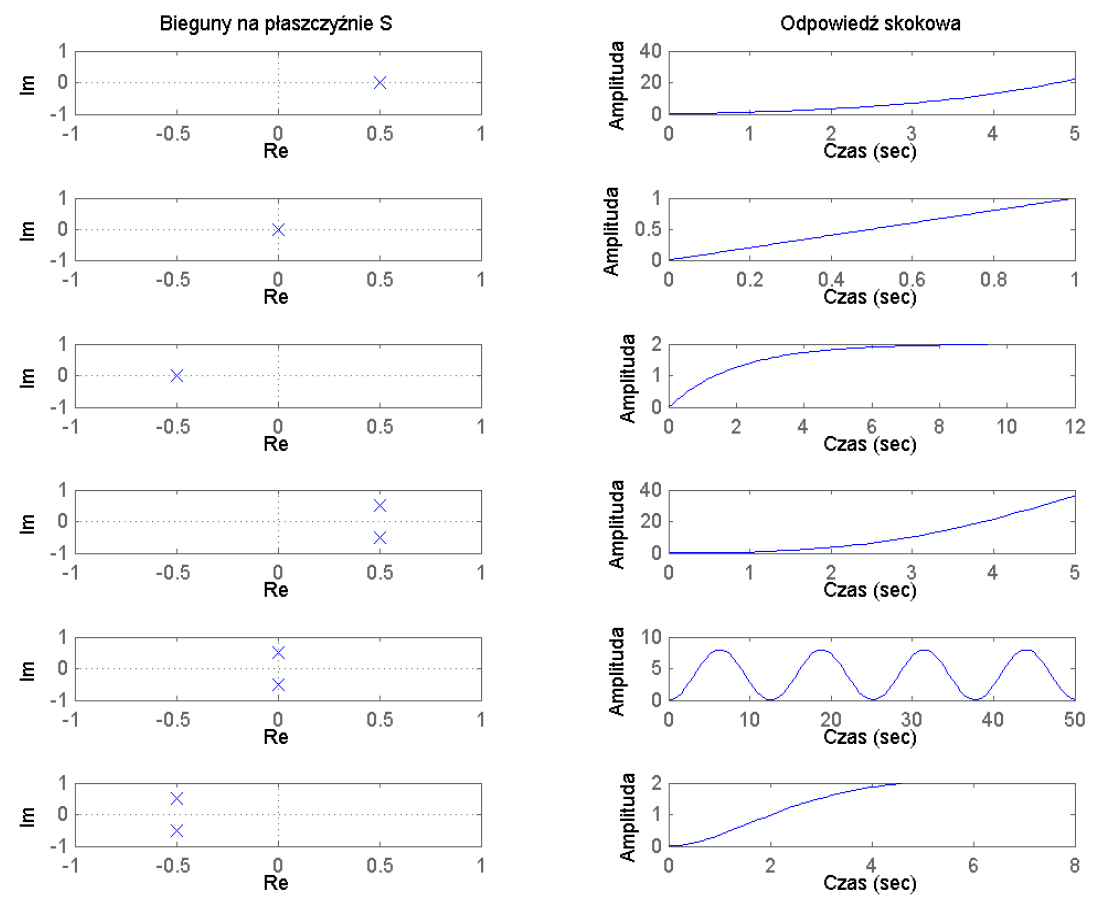
\includegraphics[scale=0.2]{tabela.png}
	\end{itemize}
	
\end{frame}

\begin{frame}\frametitle{Wprowadzenie}\framesubtitle{}
	W dziedzinie Laplace'a wnioskujemy:
	\begin{enumerate}
		\item Jeżeli pierwiastki równania charakterystycznego leżą w lewej półpłaszczyźnie zespolonej, to układ jest stabilny.
		
		\item Jeżeli wszystkie pierwiastki leżą na osi rzeczywistej to układ jest przetłumiony lub tłumiony krytycznie.
		
		\item Im większe ujemne wartości pierwiastków równania charakterystycznego układu tym szybsza jest dynamika układu.
		
		\item Im bliżej osi urojonej leżą pierwiastki równania charakterystycznego tym większy wpływ na dynamikę mają one.
		
		\item Im większe współczynniki części urojonej pary sprzężonej pierwiastków równania charakterystycznego tym bardziej oscylacyjny jest układ.
	\end{enumerate}
\end{frame}

\begin{frame}\frametitle{Wprowadzenie}\framesubtitle{}
	Linie pierwiastkowe - wykres pierwiastków równania charakterystycznego układu zamkniętego zależnych od wartości wzmocnienia K.
	
	Własności linii pierwiastkowych:
	\begin{enumerate}
		\item Początek linii pierwiastkowych leży w miejscu odpowiadającym biegunom układu otwartego.
		
		\item Linie kończą się w zerach transmitacji.
		
		\item Liczba linii pierwiastkowych odpowiada liczbie biegunów.
		
		\item Linie będące wykresami pierwiastków zespolonych występują w postaci par sprzężonych.
	\end{enumerate}
\end{frame}

\begin{frame}\frametitle{Wprowadzenie}\framesubtitle{}
	Częstotliwość własna - szybkość drgań układu po wytrąceniu z położenia równowagi oraz pozostawionego bez żadnego wpływu z zewnątrz. Liczbowo jest ona równa odległości biegunów od początku układu współrzędnych:
	\[
		\omega = \frac{1}{T}
	\]
\end{frame}

%-------ZADANIE 1-----------

\begin{frame}\frametitle{Zadanie 1}\framesubtitle{Badanie linii pierwiastkowych}
Zbadaj wykresy linii pierwiastkowych dla następujących układów:
\[
a) ~~ G(s) = \frac{1}{(s+1)(5s+1)}
\]

\[
b) ~~ G(s) = \frac{0,5s + 1}{(s+1)(5s+1)}
\]

\[
c) ~~ G(s) = \frac{1}{(s+1)(5s+1)(0,5s + 1)}
\]
\end{frame}

%-----------A----------------
%-----------B----------------
%-----------C----------------

\begin{frame}[fragile]\frametitle{Zadanie 1}\framesubtitle{Badanie linii pierwiastkowych - algorytm i kod}

\begin{lstlisting}[centering]
% Zadanie 1a
% Utworzenie ukladu dynamicznego
sys = zpk([],[0 -1 -5], 5);

% Narysowanie linii pierwiastkowych
rlocus(sys);

%-----------------------------------

% Zadanie 1b
% Utworzenie ukladu dynamicznego
sys = zpk(-2, [-1 -1/5], 1/5);

% Narysowanie linii pierwiastkowych
rlocus(sys);

%-----------------------------------

% Zadanie 1c
% Utworzenie ukladu dynamicznego
sys = zpk([], [-1 -1/5 -2], 10/25);

% Narysowanie linii pierwiastkowych
rlocus(sys);

% Obliczenie K dla zadanego kata
[K, bieguny] = rlocfind(sys);

\end{lstlisting}

\end{frame}

\begin{frame}\frametitle{Zadanie 1a}\framesubtitle{Badanie linii pierwiastkowych - wykonanie}

\centering	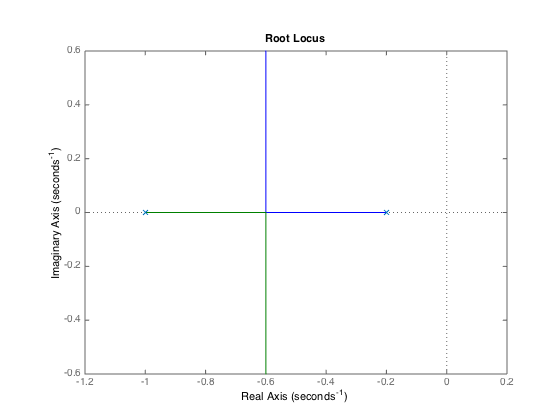
\includegraphics[scale=0.45]{zadanie1_a.png}

\end{frame}

\begin{frame}\frametitle{Zadanie 1b}\framesubtitle{Badanie linii pierwiastkowych - wykonanie}
	
	\centering	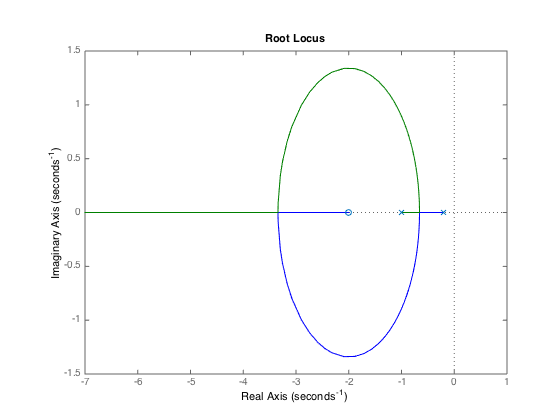
\includegraphics[scale=0.45]{zadanie1_b.png}
	
\end{frame}

\begin{frame}\frametitle{Zadanie 1c}\framesubtitle{Badanie linii pierwiastkowych - wykonanie}
	
	\centering	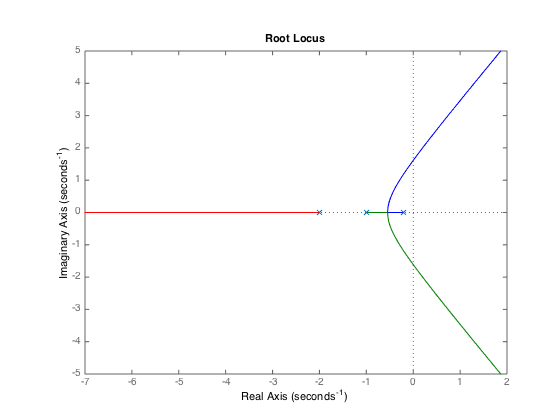
\includegraphics[scale=0.45]{zadanie1_c1.png}
	
\end{frame}

\begin{frame}\frametitle{Zadanie 1c}\framesubtitle{Badanie linii pierwiastkowych - wykonanie}
	
	\centering	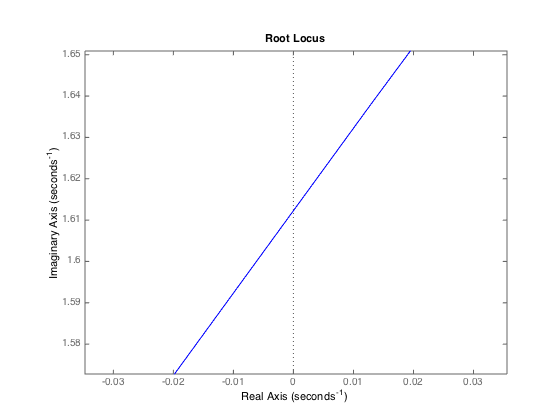
\includegraphics[scale=0.45]{zadanie1_c2.png}
	
\end{frame}

\begin{frame}\frametitle{Zadanie 1c}\framesubtitle{Badanie linii pierwiastkowych - wykonanie}
	
	\centering	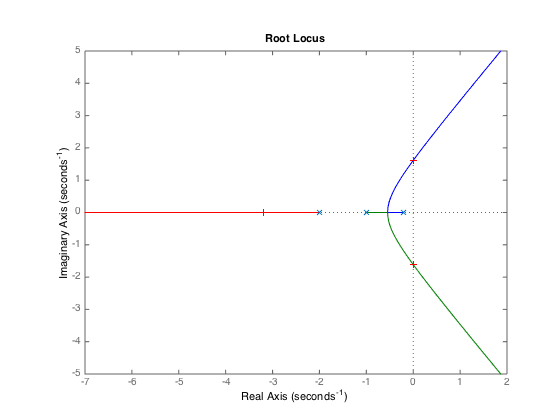
\includegraphics[scale=0.45]{zadanie1_c.png}
	
\end{frame}

\begin{frame}[fragile]\frametitle{Zadanie 1c}\framesubtitle{Badanie linii pierwiastkowych - wykonanie}
	
Z sytemu z podpunktu c wynika, że układ staje się niestabilny dla wzmocnienia krytycznego równego:
	
\begin{lstlisting}
>> zadanie_1.m
Select a point in the graphics window
	
	selected_point =
	
	0.0002 + 1.6126i

\end{lstlisting}	
\end{frame}


%-------ZADANIE 2-----------
%-----------A---------------

\begin{frame}\frametitle{Zadanie 2}\framesubtitle{Dobór regulatora proporcjonalnego}
	Dany jest układ:
	\[
	G(s) = \frac{1}{s(s+1)(0.2s+1)}
	\]
    \begin{enumerate}[a)]
        \item Wykorzystując poznane narzędzia dobierz regulator proporcjonalny (wzmocnienie K) aby układ zamknięty miał współczynnik tłumienia $\xi = 0.707$ (wtedy $\phi = 45\degres$). Narysuj odpowiedź skokową układu zamkniętego.
        
        \centering{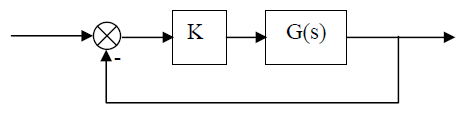
\includegraphics[scale=0.65]{uklad-2.png}}
        
        %\item Dodaj do układu kompensator (człon przyspieszająco-opóźniający fazę) o transmitancji:
        %\[
        %	G_c(s) = \frac{(s+1)}{(0.1s+1)}
        %\]
        %czyli utwórz następujący układ:
    \end{enumerate}
\end{frame}

\begin{frame}[fragile]\frametitle{Zadanie 2a}\framesubtitle{Dobór regulatora proporcjonalnego - algorytm i kod}
	\begin{lstlisting}
% Utworzenie ukladu dynamicznego
sys = zpk([],[0 -1 -5], 5);

% Narysowanie linii pierwiastkowych
rlocus(sys);

% Pomocnicza linia pod zadanym katem 45 stopnii
line([0 -15], [0 15]);           

% Zatrzymanie w celu przyblizenia
pause();                            

% Obliczenie K dla zadanego kata
[K, bieguny] = rlocfind(sys);       

% Zamkniecie ukladu dynamicznego
sys_zamk = feedback(K * sys, 1);    

% Odpowiedz ukladu zamknietego na skok jednostkowy
step(sys_zamk);                     

% Wyswietlenie K w tytule wykresu
title(['Step response, K = ' num2str(K)]);
	\end{lstlisting}
\end{frame}

\begin{frame}\frametitle{Zadanie 2a}\framesubtitle{Dobór regulatora proporcjonalnego - wykonanie}
\centering	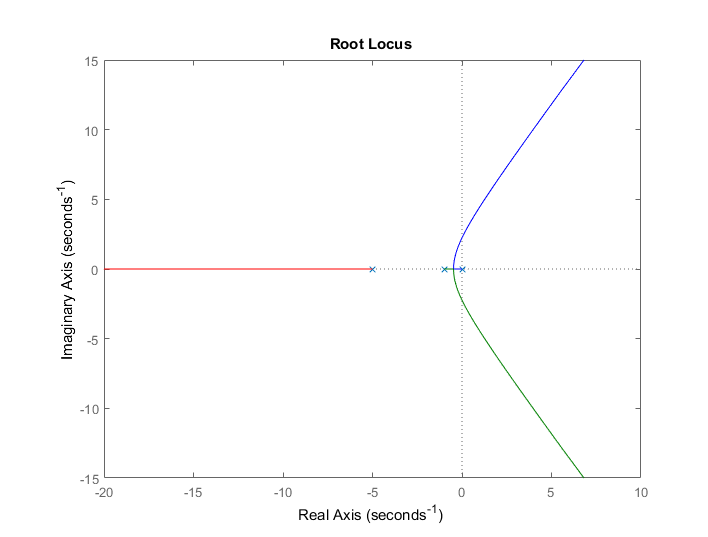
\includegraphics[scale=0.5]{a-rlocus-bez-linii.png}
\end{frame}

\begin{frame}\frametitle{Zadanie 2a}\framesubtitle{Dobór regulatora proporcjonalnego - wykonanie}
\centering	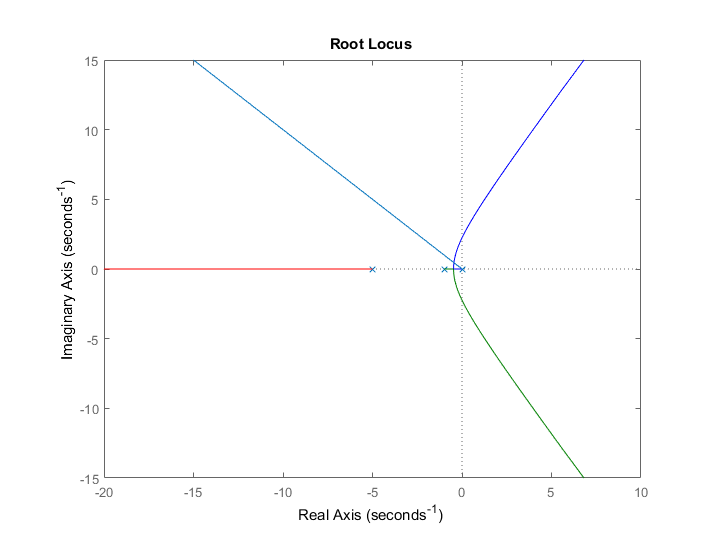
\includegraphics[scale=0.5]{a-rlocus.png}
\end{frame}

\begin{frame}\frametitle{Zadanie 2a}\framesubtitle{Dobór regulatora proporcjonalnego - wykonanie}
\centering	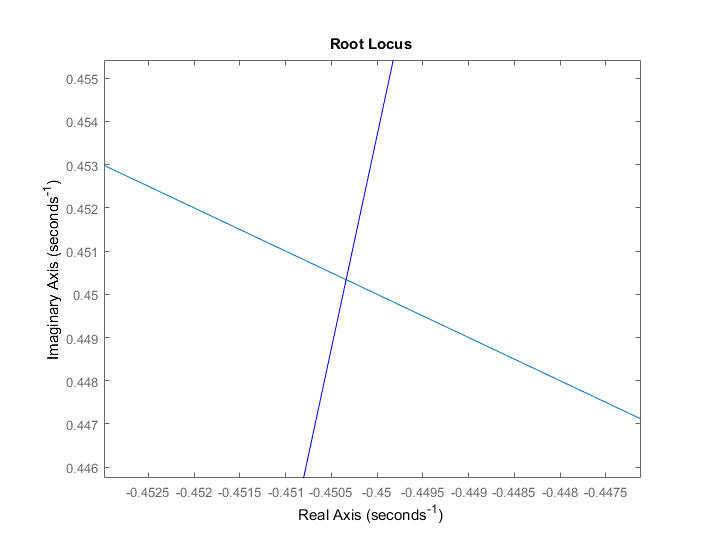
\includegraphics[scale=0.5]{a-przyblizenie.png}
\end{frame}

\begin{frame}\frametitle{Zadanie 2a}\framesubtitle{Dobór regulatora proporcjonalnego - wykonanie}
\centering	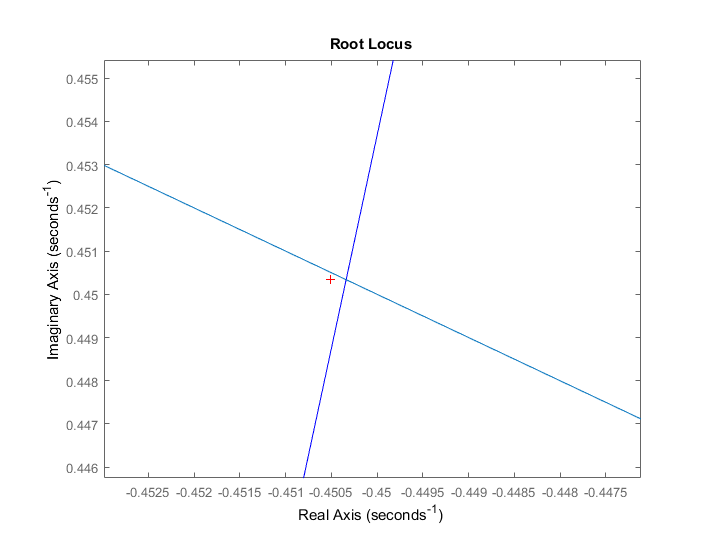
\includegraphics[scale=0.5]{a-rlocfind.png}
\end{frame}

\begin{frame}\frametitle{Zadanie 2a}\framesubtitle{Dobór regulatora proporcjonalnego - wykonanie}
\centering	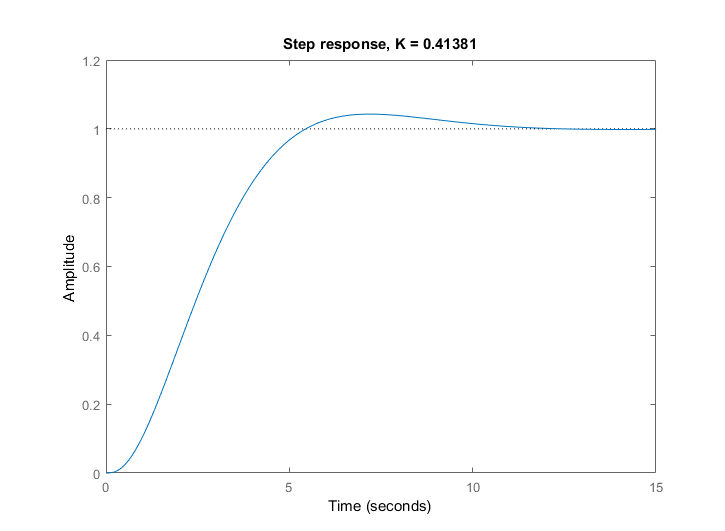
\includegraphics[scale=0.5]{a-sys-zamk-k.png}
\end{frame}

%-----------B------------

\begin{frame}\frametitle{Zadanie 2b}\framesubtitle{Dobór regulatora proporcjonalnego z kompensatorem}
	\begin{enumerate}[b)]
		\item Dodaj do układu kompensator (człon przyspieszająco-opóźniający fazę) o transmitancji:
		\[
			G_c(s) = \frac{(s+1)}{(0.1s+1)}
		\]	
		czyli utwórz następujący układ:
		
		
		\centering{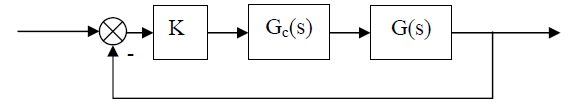
\includegraphics[scale=0.65]{uklad-2-b.png}}
		
		
		\flushleft Dobierz wzmocnienie K aby układ zamknięty miał taki sam współczynnik tłumienia jak w punkcie a). Narysuj odpowiedź skokową układu zamkniętego.
	\end{enumerate}
\end{frame}

\begin{frame}[fragile]\frametitle{Zadanie 2b}\framesubtitle{Dobór regulatora proporcjonalnego z kompensatorem - algorytm i kod}
	\begin{lstlisting}
% Oryginalny system dynamiczny
sys = zpk([],[0 -1 -5], 5);
% Utworzenie kompensatora
Gc = zpk(-1, -10, 1/10);
% Utworzenie systemu zastepczego
system_zastepczy = series(sys, Gc);
% Narysowanie linii pierwiastkowych ukladu zastepczego
rlocus(system_zastepczy);
% Narysowanie linii pomocniczej
line([0, -15], [0, 15]);
% Zatrzymanie wykonywania w celu przyblizenia
pause();
% Obliczenie wzmocnienia dla ukladu zastepczego
[K, bieguny] = rlocfind(system_zastepczy);
% Stworzenie ukladu zamknietego
sys_zamk_b = feedback(K * system_zastepczy, 1);
% Odpowiedz ukladu zastepczego na skok jednostkowy
step(sys_zamk_b);
% Wyswietlenie K w tytule wykresu
title(['Step response, K = ' num2str(K)]);
	\end{lstlisting}
\end{frame}

\begin{frame}\frametitle{Zadanie 2b}\framesubtitle{Dobór regulatora proporcjonalnego z kompensatorem - wykonanie}
\centering	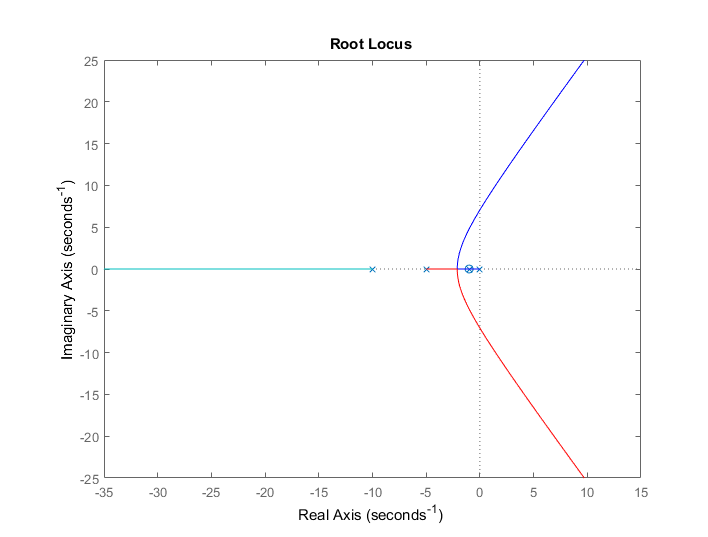
\includegraphics[scale=0.5]{b-rlocus-bez-linii.png}
\end{frame}

\begin{frame}\frametitle{Zadanie 2b}\framesubtitle{Dobór regulatora proporcjonalnego z kompensatorem - wykonanie}
\centering	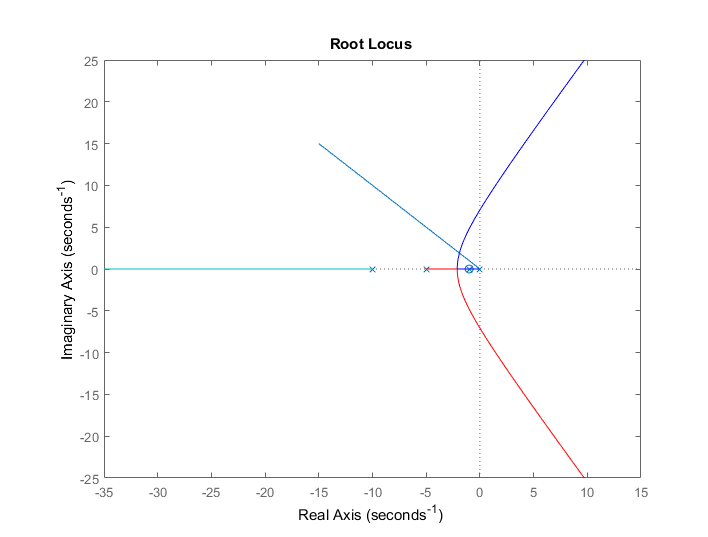
\includegraphics[scale=0.5]{b-rlocus.png}
\end{frame}

\begin{frame}\frametitle{Zadanie 2b}\framesubtitle{Dobór regulatora proporcjonalnego z kompensatorem - wykonanie}
\centering	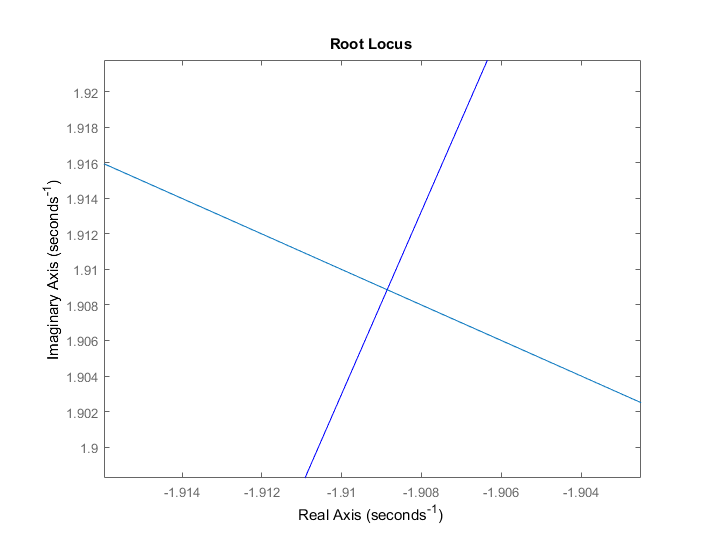
\includegraphics[scale=0.5]{b-przyblizenie.png}
\end{frame}

\begin{frame}\frametitle{Zadanie 2b}\framesubtitle{Dobór regulatora proporcjonalnego z kompensatorem - wykonanie}
\centering	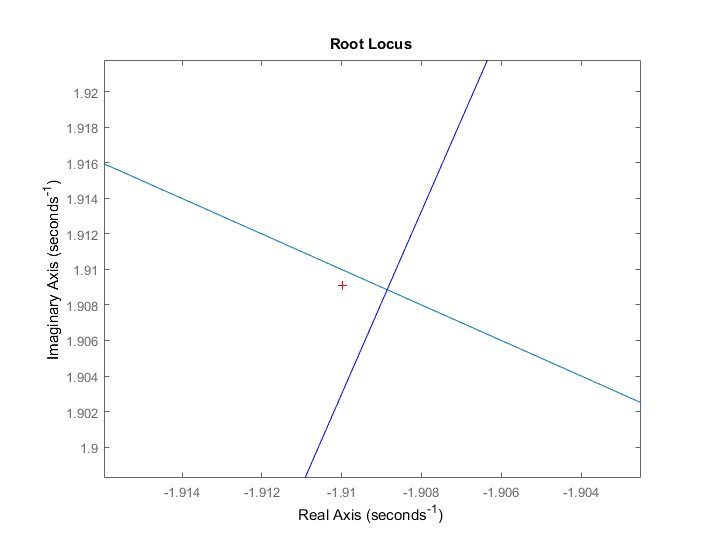
\includegraphics[scale=0.5]{b-rlocfind.png}
\end{frame}

\begin{frame}\frametitle{Zadanie 2b}\framesubtitle{Dobór regulatora proporcjonalnego z kompensatorem - wykonanie}
\centering	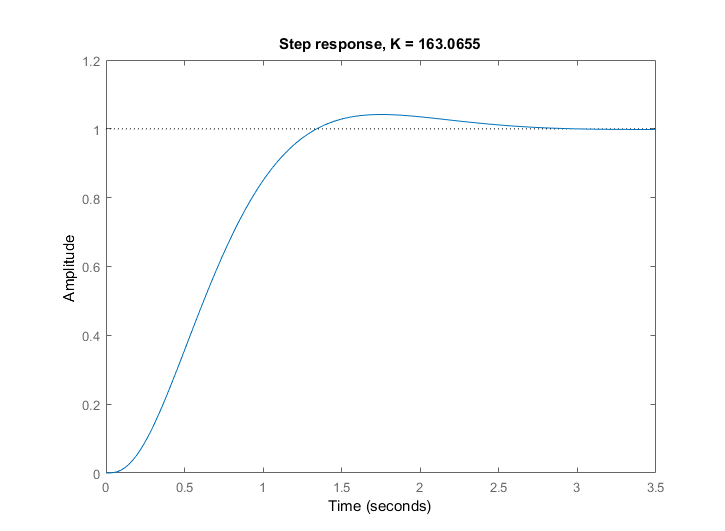
\includegraphics[scale=0.5]{b-sys-zamk-k.png}
\end{frame}

%------------OBA-------------
\begin{frame}\frametitle{Zadanie 2}\framesubtitle{Dobór regulatora proporcjonalnego - porównanie}
\centering	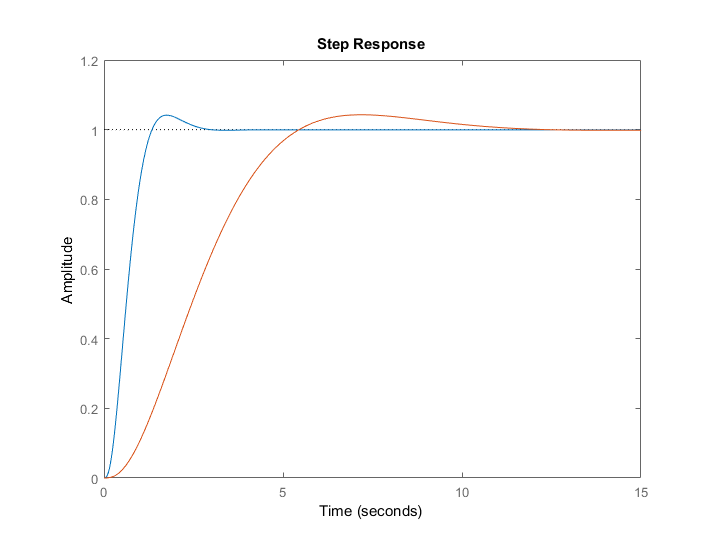
\includegraphics[scale=0.5]{step-oba.png}
\end{frame}

\begin{frame}\frametitle{Zadanie 2}\framesubtitle{Dobór regulatora proporcjonalnego - porównanie}
Z uzyskanych systemów za pomocą polecenia \texttt{pole} obliczone zostają bieguny. Pary sprzężone wynoszą odpowiednio:

\begin{itemize}
	\item Układ a: $ -0.4505 \pm 0.4504i $ 
	\item Układ b: $ -1.91 \pm 1.9091i $
\end{itemize}

Częstotliwości własne:
\begin{itemize}
	\item Układ a: $ |-0.4505 \pm 0.4504| \approx 0.0001 $
	\item Układ b: $ |-1.91 \pm 1.0901| \approx 0.8199 $
\end{itemize}


\end{frame}

\begin{frame}\frametitle{Zadanie 2}\framesubtitle{Dobór regulatora proporcjonalnego - wnioski}
	\begin{itemize}
		\item Układ zamknięty z zadanym współczynnikiem tłumienia, z kompensatorem oraz bez niego jest stabilny.
		\item Dodanie kompensatora do systemu spowodowało polepszenie właściwości dynamicznych układu - szybszą stabilizację.
		\item Układ b wykonuje szybsze drgania w stanie stabilnym.
	\end{itemize}
\end{frame}

\begin{frame}\frametitle{Bibliografia}\framesubtitle{}
	\begin{itemize}
		\item \textit{,,Metoda projektowania układów regulacji za pomocą linii pierwiastkowych''} - dr inż. Maciej Klemiato
		
		\item Wikipedia: hasło \textit{,,Częstość własna''}
		
		\item berleburger.com: hasło \textit{,,Częstotliwość własna''}
	\end{itemize}
\end{frame}

\end{document}
